%! TEX root = ./main.tex

\section{Localization}
\begin{itemize}
    \item Problems:
        \begin{itemize}
            \ides{Position tracking:} Keep track of known location
            \ides{Global localization:} Localize without initial location
            \ides{Kidnapping robot problem:} Robot is moved to new location
        \end{itemize}
    \ides{Map Representation}
        \begin{itemize}
            \item Known a priori or build by robot
            \ides{Types:}
                \begin{itemize*}
                    \item Architecture map
                    \item Finite/infinite set of lines
                    \item Exact cell decomposition
                    \item Fixed cell decomposition
                    \item Topological map
                \end{itemize*}
        \end{itemize}
    \ides{Belief Representation}
        \begin{itemize}
            \item Uncertain due to error $\implies$ probabilistic localization
            \ides{Continuous:}
                \begin{itemize*}
                    \item Precision bound by sensor data
                    \item Typically single hypotheses ($\implies$ danger of getting lost)
                \end{itemize*}
            \ides{Discretized:}
                \begin{itemize*}
                    \item Precision bound by discretization resolution
                    \item Typically multiple hypotheses
                    \item High resource demands
                \end{itemize*}
            \ides{Types:}
                \begin{itemize*}
                    \item Continuous map with single hypotheses prob. dist. $p(x)$
                    \item Continuous map with multiple hypotheses prob. dist. $p(x)$
                    \item Discretized metric map (grid $k$) with prob. dist. $p(x)$
                    \item Discretized topological map (nodes $n$) with prog. dist. $p(x)$
                \end{itemize*}
        \end{itemize}
    \ides{Odometry}
        \begin{itemize}
            \item Process of calculating current position by using previous position and measured motion of last time step
            \ides{Differential Drive Robot:} $p_t = f(p_{t - 1}, u_t) =
    \begin{bmatrix}
        x_{t - 1}\\
        y_{t - 1}\\
        \theta_{t - 1}
    \end{bmatrix} +
    \begin{bmatrix}
        \frac{\Delta S_r + \Delta S_l}{2} \cos(\theta_{t - 1} + \frac{\Delta S_r - \Delta S_l}{2b})\\
        \frac{\Delta S_r + \Delta S_l}{2} \sin(\theta_{t - 1} + \frac{\Delta S_r - \Delta S_l}{2b})\\
        \frac{\Delta S_r - \Delta S_l}{b}
    \end{bmatrix}, \linebreak b = \text{Distance between wheels}$
            \ides{Error Model:}
                \begin{itemize}
                    \ides{Error Propagation:} $\Sigma_{p_t} = F_{p_{t-1}} \Sigma_{p_{t-1}} F_{p_{t-1}}^\transpose + F_{\Delta S} \Sigma_{\Delta S} F_{\Delta S}^\transpose$
                    \ides{Error Model:} $\Sigma_{\Delta S} =
                        \begin{pmatrix}
                            k_r |\Delta S_r | & 0\\
                            0 & k_l |\Delta S_l|
                        \end{pmatrix}$
                    \item with $F_{x/y} = \bigtriangledown_{x/y} f$
                \end{itemize}
        \end{itemize}
\end{itemize}

\subsection{Map-Based Localization}
\begin{itemize}
    \item Estimate position using perceived information and a map
    \ides{Terminology:}
        \begin{itemize*}
            \ides{$\mathbf{x_t}$:} robot location at time $t$
            \ides{$\mathbf{u_t}$:} proprioceptive sensor reading at time $t$
            \ides{$\mathbf{z_t}$:} exteroceptive sensor reading (observation) at time $t$
            \ides{$\mathbf{M}$}$= \{m_0, m_1, \dots, m_{n-1}\}$ true map of the environment with $n$ features
            \ides{$\mathbf{\text{bel}(x_t)}$}$= p(x_t \mid z_{1 \to t}, u_{1 \to t})$
            \ides{$\mathbf{\overline{\text{bel}}(x_t)}$}$= p(x_t \mid z_{1 \to t - 1}, u_{1 \to t})$
        \end{itemize*}
    \ides{Requirements}
        \begin{itemize}
            \item Initial probability distribution $\text{bel}(x_0)$
            \item Map $M = \{m_0, m_1, \dots, m_n\}$ of the environment
            \item Proprioceptive and exteroceptive data $u_t$ and $z_t$
            \item Probabilistic motion model $p(x_t \mid u_t, M)$
                \begin{itemize}
                    \item Derived from the robots kinematics
                \end{itemize}
            \item Probabilistic measurement model $p(z_t \mid x_t, M)$
                \begin{itemize}
                    \item Derived from the exteroceptive sensor model
                \end{itemize}
        \end{itemize}
    \ides{Steps}
        \begin{itemize}
            \item[0)] Robot is placed somewhere in the environment
            \item[S1)] \textbf{Prediction/Action Update (ACT):} Move and estimate position using proprioceptive sensors
                \begin{itemize}
                    \item Uncertainty grows
                \end{itemize}
            \item[S2)] \textbf{Perception/Measurement Update (SEE):} Make observation using exteroceptive sensors
                \begin{itemize}
                    \item Uncertainty shrinks
                \end{itemize}
        \end{itemize}
\end{itemize}
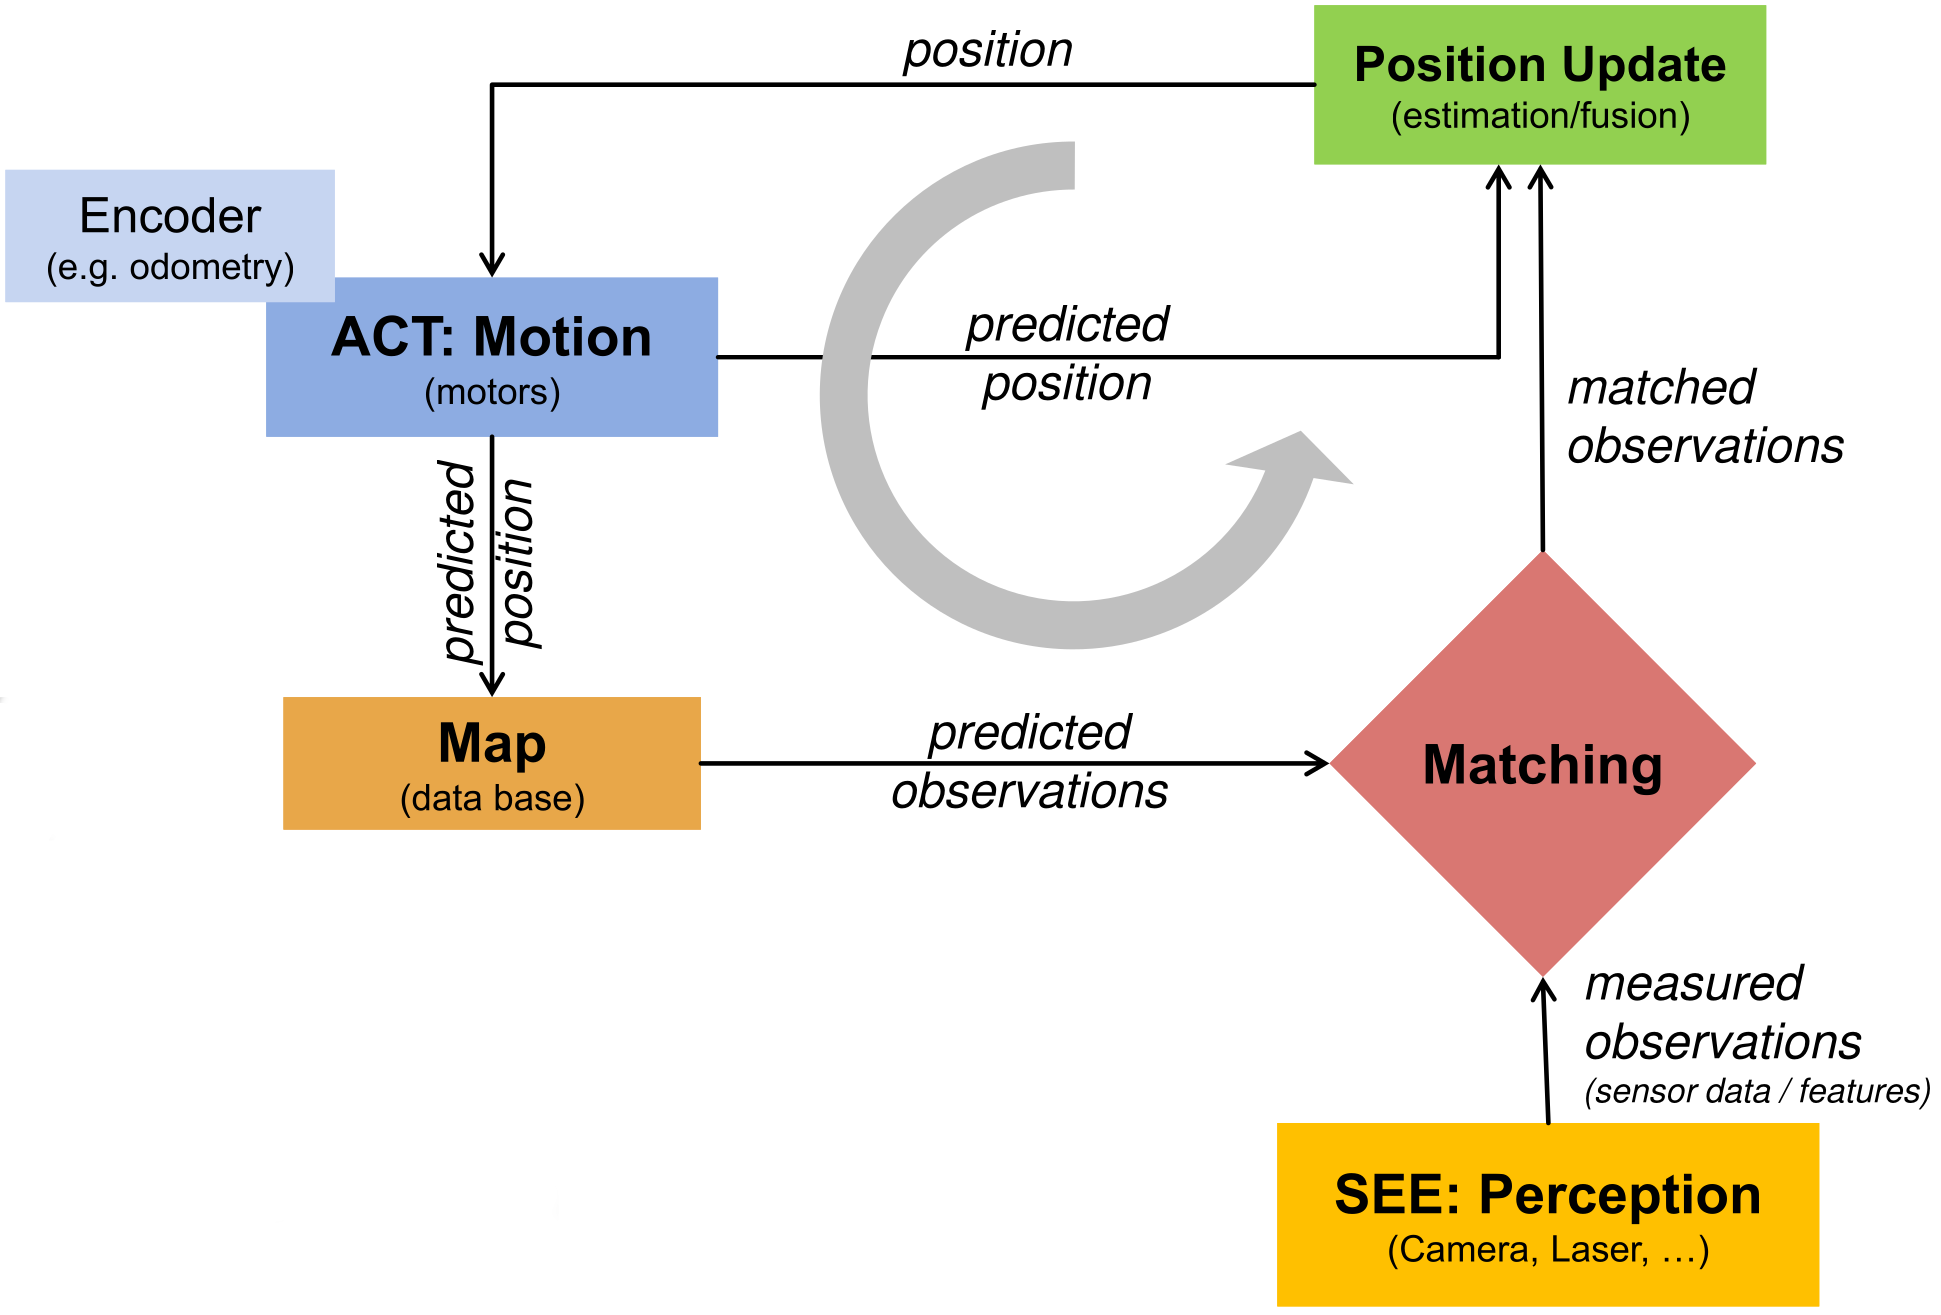
\includegraphics[width=\linewidth]{./Figures/05_LocalisationCycle.png}

\subsubsection{Markov Localization}
\begin{itemize}
    \ides{Solves:}
        \begin{itemize*}
            \item Global localization
            \item Position tracking
            \item Kidnapped robot
        \end{itemize*}
    \item Discretized pose representation $x_t$
    \item $\text{bel}(x_t)$ is representation by arbitrary prob. density function
        \begin{itemize}
            \item Multiple hypotheses
        \end{itemize}
    \ides{Markov Assumption:} $\text{bel}(x_t) = p(x_t \mid x_0, u_{0 \to t}, z_{0 \to t}) = p(x_t \mid x_{t - 1}, u_t, z_t)$
    \ides{Steps:}
\end{itemize}
\begin{algorithmic}
    \FORALL{$x_t$}
        \STATE \textit{S1)} \textbf{ACT:} $\overline{\text{bel}}(x_t) = \sum_{x_{t-1}} p(x_t \mid u_t, x_{t - 1}) \text{bel}(x_{t-1})$
        \STATE \textit{S2)} \textbf{SEE:} $\text{bel}(x_t) = \eta p(z_t \mid x_t, M) \overline{\text{bel}}(x_t)$ with $\eta = \frac{1}{p(y)}$
    \ENDFOR
\end{algorithmic}
\begin{itemize}
    \icon Huge state space
    \icon Inefficient
    \ides{Improvements:}
        \begin{itemize*}
            \item Change of cell size
            \item Adaptive cell size
            \ides{Randomized Sampling:} Approximation of belief state by a representative subset of possible locations. Higher density around peak points
        \end{itemize*}
\end{itemize}

\subsubsection{Extended Kalman Filter (EKF) Localization}
\begin{itemize}
    \ides{Solves:}
        \begin{itemize*}
            \item Position tracking
        \end{itemize*}
    \item $\text{bel}(x_t)$, motion model and measurement model is represented by a normal distribution
        \begin{itemize}
            \item Single hypotheses
        \end{itemize}
    \ides{Steps:}
        \begin{itemize}
            \item[S1)] \textbf{Prediction Update}
                \begin{itemize}
                    \item New position: $\hat x_t = f(x_{t-1}, u_t)$
                    \item Position uncertainty: $\hat P_t = F_x P_{t-1} F_x^\transpose + F_u Q_t F_u^\transpose$
                    \item
                        \begin{itemize}
                            \ides{$\mathbf{P_{t - 1}}$:} Covariance of the previous state $x - 1$
                            \ides{$\mathbf{Q_t}$:} Covariance of motion model noise
                            \ides{$\mathbf{F_{x/u}}$:} Jacobian w.r.t. $x/u$
                        \end{itemize}
                \end{itemize}
            \item[S2)] \textbf{Measurement Update}
                \begin{itemize}
                    \item[1)] \textbf{Observation:} Obtain set of observation $z_t^i$ with covariance $R_t^i, i=1 \dots n$
                    \item[2)] \textbf{Measurement Prediction:} Predict feature observations $\hat z_t^j = h^j(\hat x_t, m^j)$ and compute its Jacobian $H^j$ w.r.t $\hat x_t$

                    \item[3)] \textbf{Matching:}
                        \begin{itemize}
                            \item Compute the innovation $v_t^{ij} = [z_t^i - \hat z_t^j]$
                            \item Compute the innovation covariance $\Sigma_{IN_t}^{ij} = H^j \hat P_t {H^j}^\transpose + R_t^i$
                            \item Find matches with a validation gate $g$
                                \begin{itemize}
                                    \item Mahalanobis distance: ${v_t^{ij}}^\transpose (\Sigma_{IN_t}^{ij})^{-1} v_t^{ij} \le g^2$
                                \end{itemize}
                        \end{itemize}
                    \item[4)] \textbf{Estimation:}
                        \begin{itemize}
                            \item Stack validated observations into $z_t$, corresponding innovations into $v_t$, measurement Jacobians into $H_t$ and $R_t = \mathrm{diag}(R_t^i)$
                            \item Compute composite innovation covariance $\Sigma_{IN_t}$
                            \item For each match, update position estimate $x_t = \hat x_t + K_t v_t$
                            \item For each match, update covariance $P_t = \hat P_t - K_t \Sigma_{IN_t}K_t^\transpose$
                                \begin{itemize}
                                    \ides{Kalman Gain:} $K_t = \hat P_t H_t^\transpose (\Sigma_{IN_t})^{-1}$
                                \end{itemize}
                        \end{itemize}
                \end{itemize}
        \end{itemize}
    \ipro Precise
    \ipro Efficient
    \icon Robot may get lost
\end{itemize}

\subsection{Simultaneous Localization and Mapping (SLAM)}
\begin{itemize}
    \item Create map and localize in parallel only using proprioceptive and exteroceptive sensor data
    \ides{Terminology:}
        \begin{itemize*}
            \ides{$\mathbf{x_t}$:} robot location at time $t$
            \ides{$\mathbf{X_t}$}$=\{x_0, x_1, \dots, x_t\}$ robot path till time $t$
            \ides{$\mathbf{u_t}$:} motion between $t-1$ and $t$
            \ides{$\mathbf{U_t}$}$=\{u_0, u_1, \dots, u_t\}$ sequence of relative motions till time $t$
            \ides{$\mathbf{z_t}$:} landmark observation at time $t$
            \ides{$\mathbf{Z_t}$}$=\{z_0, z_1, \dots, z_t\}$ sequence of landmark observations till time $t$
            \ides{$\mathbf{z_t}$:} exteroceptive sensor reading (observation) at time $t$
            \ides{$\mathbf{M}$}$= \{m_0, m_1, \dots, m_{n-1}\}$ true map of the environment with $n$ landmarks
        \end{itemize*}
    \ides{Full SLAM:} Reconstruct full path $p(X_t, M \mid Z_t, U_t)$
    \ides{Online SLAM:} Reconstruct current position $p(x_t, M \mid Z_t, U_t)$
    \ides{Approaches:}
        \begin{itemize}
            \ides{Full Graph Optimisation}
                \begin{itemize}
                    \item Eliminate observations and control inputs
                    \item Solve for constraints between poses and landmarks
                    \ipro Finds globally consistent solution
                    \ipro Trajectories can be very smooth
                    \icon Sparsify graph for real-time application
                    \\ 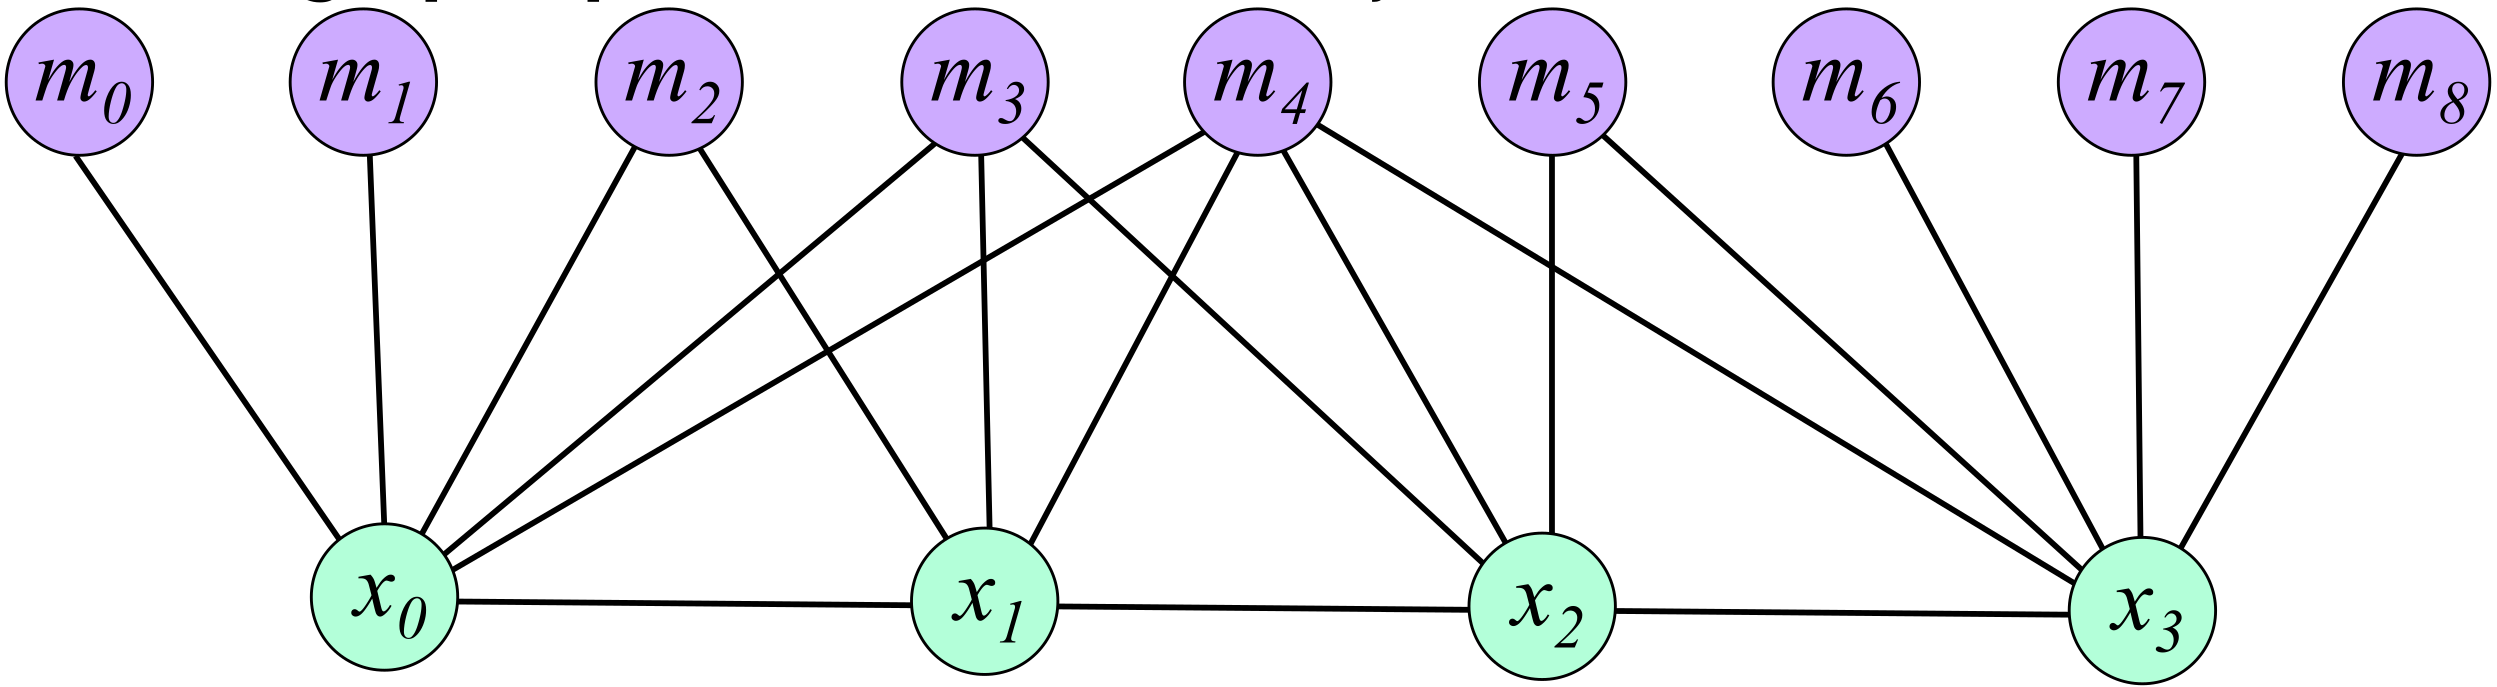
\includegraphics[width=\linewidth]{./Figures/05_SLAM_FullGraphOptimisation.png}
                \end{itemize}
            \ides{Key Frames}
                \begin{itemize}
                    \item Retain most representative poses and their dependency links
                    \item Optimize resulting graph
                    \item Example: PTAM, OKVIS, ORB-SLAM
                    \\ 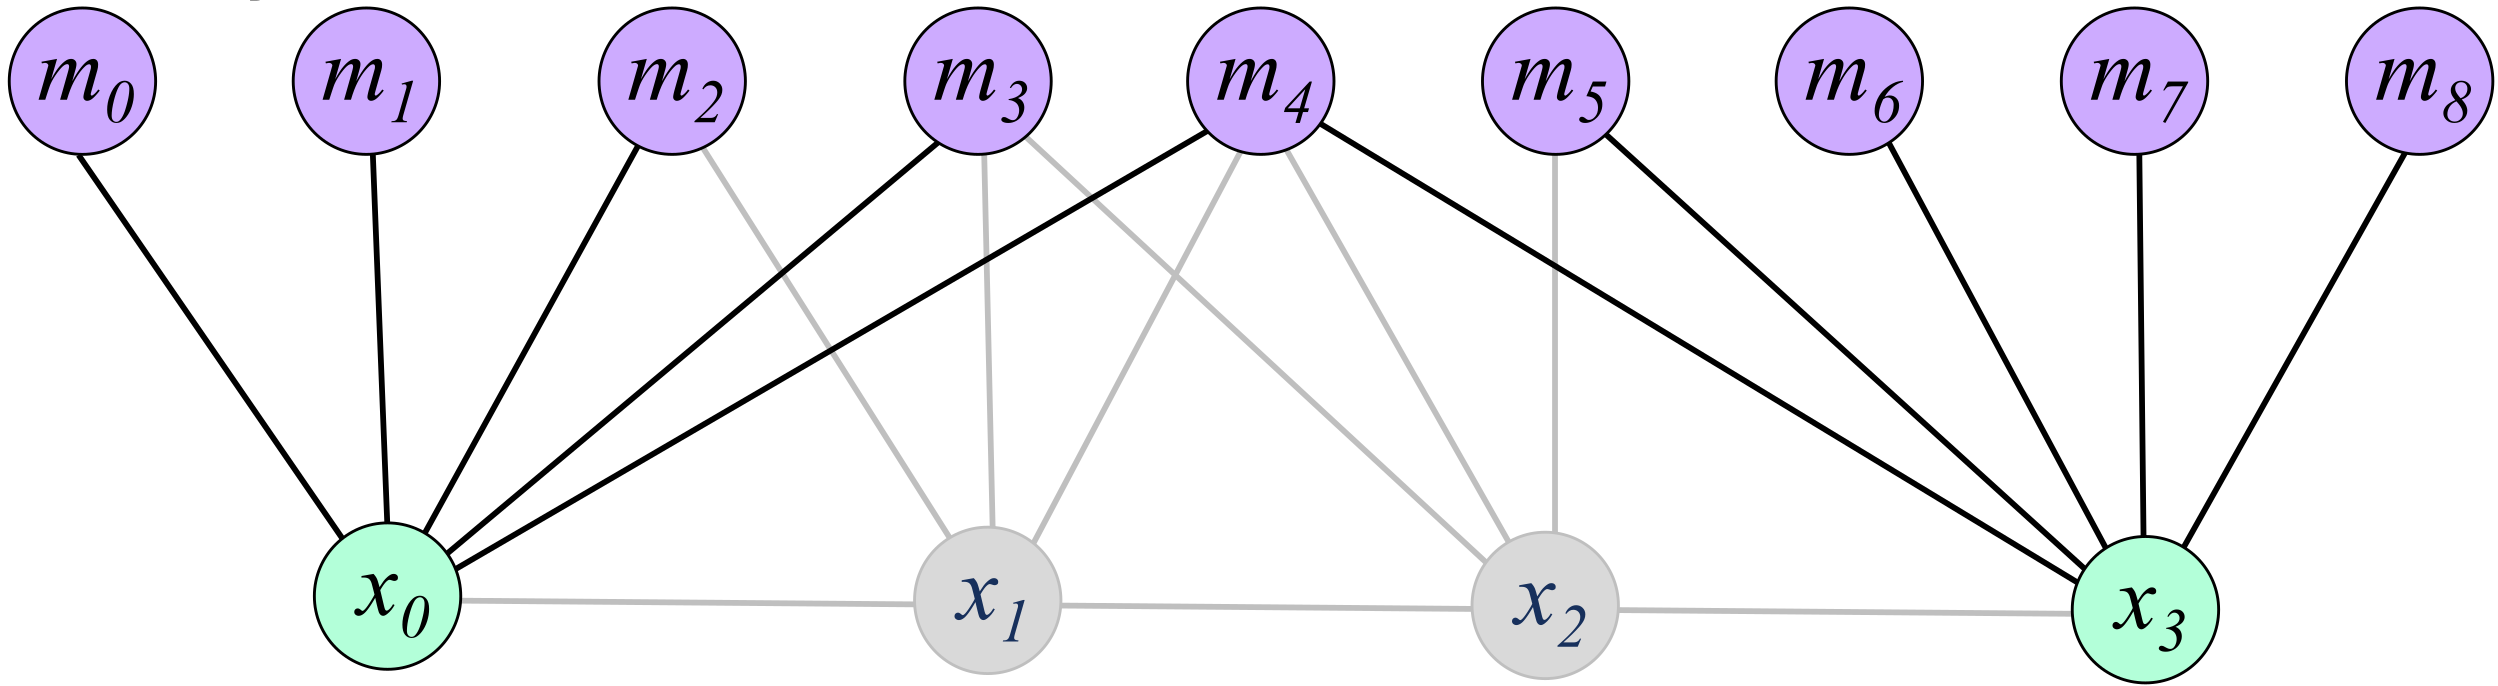
\includegraphics[width=\linewidth]{./Figures/05_SLAM_KeyFrames.png}
                \end{itemize}
            \ides{Filtering}
                \begin{itemize}
                    \item Summarize all experience w.r.t. last pose
                    \item Done using state vector and covariance matrix
                    \item Example: MonoSLAM, FastSLAM
                    \\ 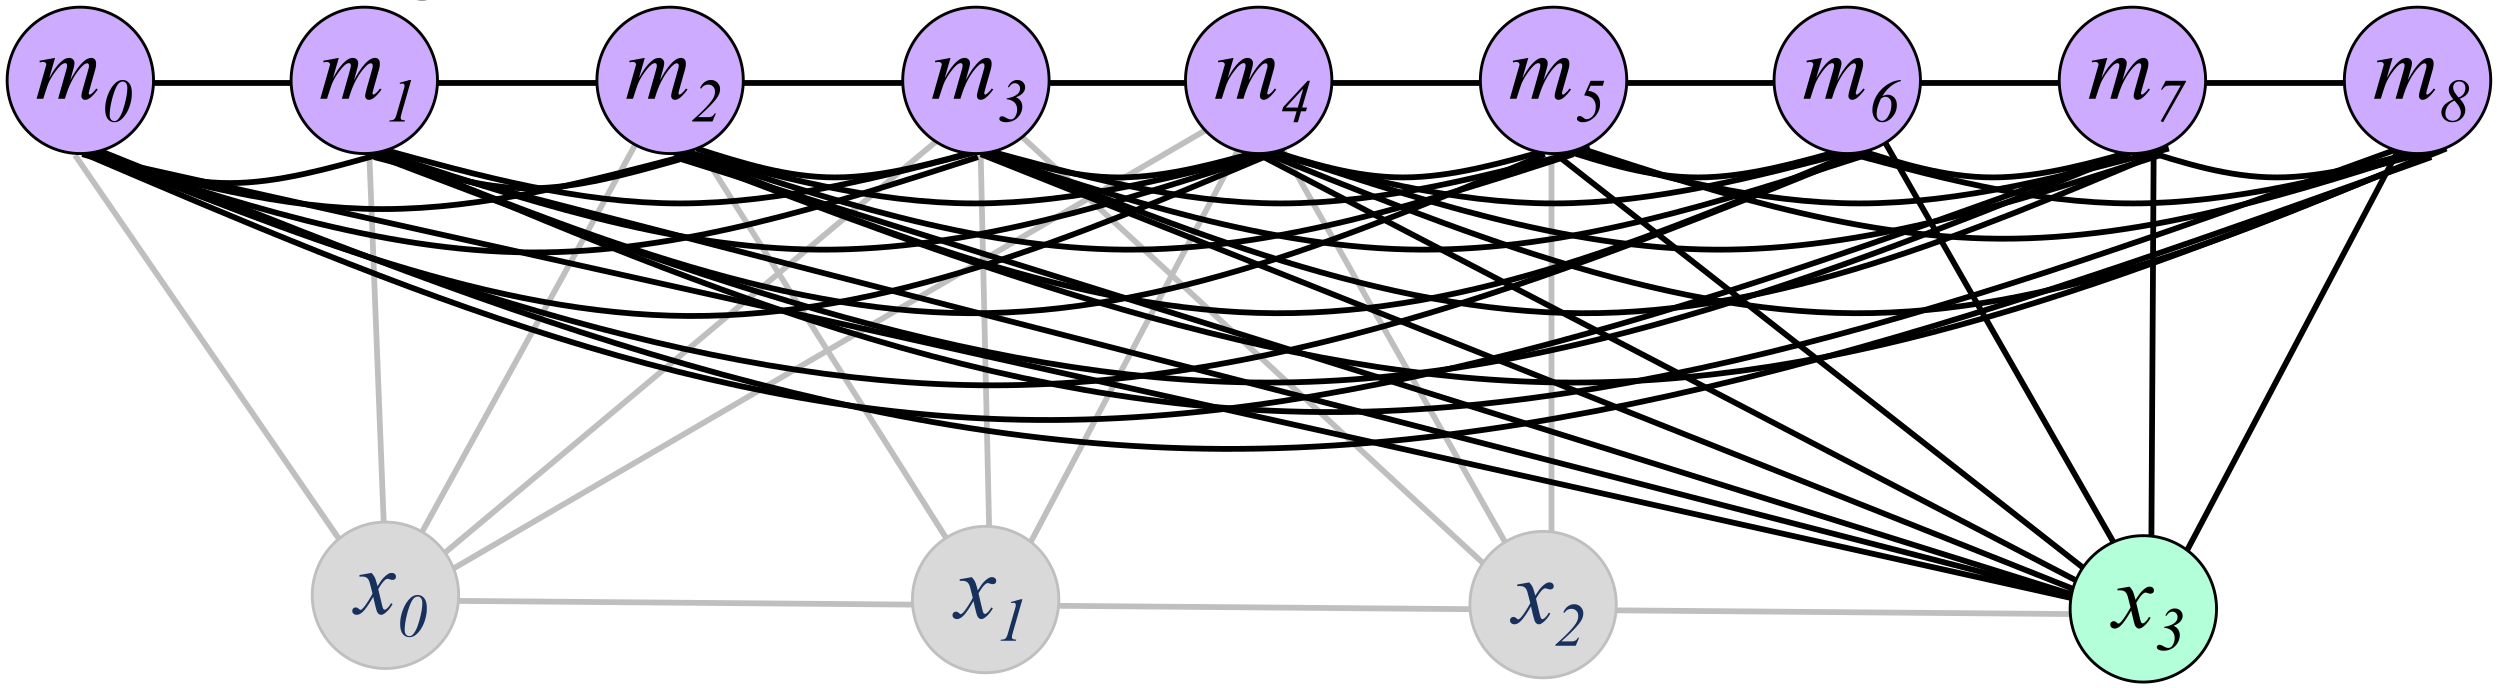
\includegraphics[width=\linewidth]{./Figures/05_SLAM_Filtering.png}
                \end{itemize}
        \end{itemize}
\end{itemize}

\subsubsection{EKF SLAM}
\begin{itemize}
    \item Example of filtering
    \item Summarizes past experience:
        \begin{itemize}
            \item Extended state vector $y_t =
                \begin{bmatrix}
                    x_t,  m_1, \cdots, m_{n-1}
                \end{bmatrix}^\transpose$
            \item Corresponding covariance $P_{y_t} =
                \begin{bmatrix}
                    P_{xx} & \cdots & P_{xm_{n-1}} \\
                    \vdots & \ddots & \vdots \\
                    P_{m_{n-1}x} & \cdots & P_{m_{n-1}m_{n-1}} \\
                \end{bmatrix}$
        \end{itemize}
    \item[S1)] \textbf{Prediction:}
        \begin{itemize}
            \item According to EKF equations
                \begin{itemize}
                    \item $\hat y_t =
                        \begin{bmatrix}
                          \hat x_t \\
                          m_i
                        \end{bmatrix} =
                        \begin{bmatrix}
                          f(x_{t-1}, u_t) \\
                          \mathbf 0
                        \end{bmatrix}$
                    \item $\hat P_{y_t} = F_y P_{y_{t-1}}F_y^\transpose + F_uQ_tF_u^\transpose$
                \end{itemize}
        \end{itemize}
    \item[S2)] \textbf{Measurement:}
        \begin{itemize}
            \item Measurement model $\hat z_i=h_i(\hat x_t, m_i)$ as in EKF localization
        \end{itemize}
    \item[S3)] \textbf{Update:}
        \begin{itemize}
            \item Update the state with actual observations $Z_{n-1}$:
            \item $y_t = \hat y_t + K_t (Z_{n-1} - h_{0:n-1}(\hat x_t, M_{n-1}))$
            \item $P_{y_t} = \hat P_{y_t} - K_t \Sigma_{IN} K_t^\transpose$
            \item Where
                \begin{itemize*}
                    \item $\Sigma_{IN} = H \hat P_{y_t} H^\transpose + R$
                    \item Kalman gain $K_t = \hat P_{y_t} H (\Sigma_{IN})^{-1}$
                \end{itemize*}
        \end{itemize}
    \item Initially, the covariance matrix is sparse (features are uncorrolated)
    \item After some time the covariance matrix becomes more dense
    \ides{MonoSLAM}
        \begin{itemize}
            \item EKF SLAM implementation
            \item Only one camera $\implies$ no proprioceptive data $\implies$ custom motion model
            \ides{Constant Velocity Motion Model}\\
                $f_v =
                \begin{bmatrix}
                  \mathbf r_\mathrm{new}^W \\
                  \mathbf q_\mathrm{new}^{WR} \\
                  \mathbf v_\mathrm{new}^W \\
                  \mathbf \omega_\mathrm{new}^W
                \end{bmatrix} =
                \begin{bmatrix}
                  \mathbf r^W + (\mathbf v^W + \mathbf V^W)\Delta t \\
                  \mathbf q^{WR} \times \mathbf q((\omega^W+\mathbf\Omega^W)\Delta t)\\
                  \mathbf v^W + \mathbf V^W\\
                  \mathbf \omega^W + \mathbf \Omega^W
                \end{bmatrix}$
            \item Unknown linear and angular accelerations cause a velocity impulse in each time step:\\
                $n =
                \begin{bmatrix}
                    \mathbf V^W\\
                    \mathbf \Omega^W
                \end{bmatrix} =
                \begin{bmatrix}
                    \mathbf a^W\Delta t\\
                    \mathbf \alpha^W\Delta t
                \end{bmatrix}$
        \end{itemize}
    \ides{Challenges}
        \begin{itemize*}
            \item Robust local motion estimation
            \item Mapping and loop-closure detection
            \item Map management and optimisation
            \item Sensitivity to incorrect data associations
            \item Tradeoff between efficiency and precision
            \item Dynamic objects
            \item Collaborative exploration
        \end{itemize*}
\end{itemize}
